% Arithmetic coding of baa with p(a)=0.6, p(b)=0.3, p(c)=0.1.
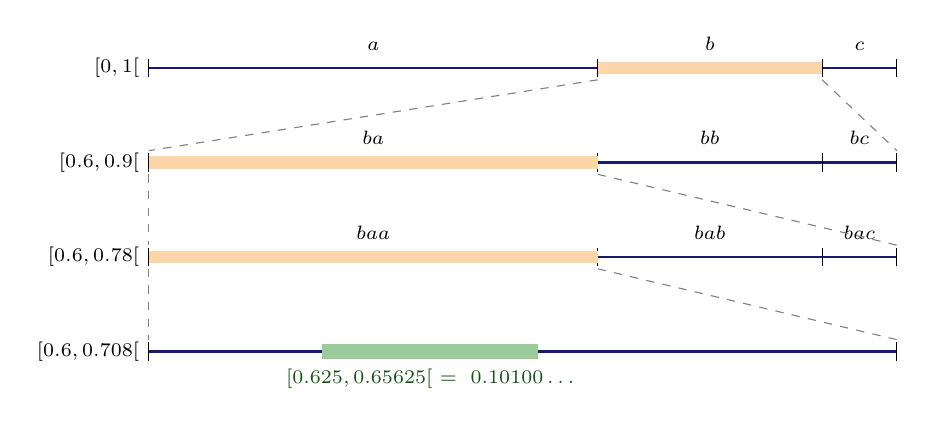
\begin{tikzpicture}[x=95mm,y=10mm,font=\scriptsize]
% level 0: [0,1)
\draw[MidnightBlue,thick] (0,0)--(1,0); \foreach \t in {0,1} \draw (\t,-0.12)--(\t,0.12);
\foreach \t/\l in {0.6/,0.9/} \draw (\t,-0.12)--(\t,0.12);
\node[above] at (0.3,0.1) {$a$}; \node[above] at (0.75,0.1) {$b$}; \node[above] at (0.95,0.1) {$c$};
\node[left] at (0,0) {$[0,1[$};
\fill[BurntOrange!30] (0.6,-0.08) rectangle (0.9,0.08);
% level 1: [0.6,0.9) magnified to full width
\begin{scope}[shift={(0,-1.2)}]
\draw[MidnightBlue,thick] (0,0)--(1,0); \foreach \t in {0,0.6,0.9,1} \draw (\t,-0.12)--(\t,0.12);
\fill[BurntOrange!30] (0,-0.08) rectangle (0.6,0.08);
\node[above] at (0.3,0.1) {$ba$}; \node[above] at (0.75,0.1) {$bb$}; \node[above] at (0.95,0.1) {$bc$};
\node[left] at (0,0) {$[0.6,0.9[$};
\end{scope}
\draw[dashed,gray] (0.6,-0.15) -- (0,-1.05); \draw[dashed,gray] (0.9,-0.15) -- (1,-1.05);
% level 2: [0.6,0.78)
\begin{scope}[shift={(0,-2.4)}]
\draw[MidnightBlue,thick] (0,0)--(1,0); \foreach \t in {0,0.6,0.9,1} \draw (\t,-0.12)--(\t,0.12);
\fill[BurntOrange!30] (0,-0.08) rectangle (0.6,0.08);
\node[above] at (0.3,0.1) {$baa$}; \node[above] at (0.75,0.1) {$bab$}; \node[above] at (0.95,0.1) {$bac$};
\node[left] at (0,0) {$[0.6,0.78[$};
\end{scope}
\draw[dashed,gray] (0,-1.35) -- (0,-2.25); \draw[dashed,gray] (0.6,-1.35) -- (1,-2.25);
% level 3: [0.6,0.708) with dyadic interval [0.625,0.65625)
\begin{scope}[shift={(0,-3.6)}]
\draw[MidnightBlue,thick] (0,0)--(1,0); \foreach \t in {0,1} \draw (\t,-0.12)--(\t,0.12);
\fill[ForestGreen!45] ({(0.625-0.6)/0.108},-0.1) rectangle ({(0.65625-0.6)/0.108},0.1);
\node[left] at (0,0) {$[0.6,0.708[$};
\node[below,ForestGreen!60!black] at ({(0.640625-0.6)/0.108},-0.1) {$[0.625,0.65625[\ =\ 0.10100\ldots$};
\end{scope}
\draw[dashed,gray] (0,-2.55) -- (0,-3.45); \draw[dashed,gray] (0.6,-2.55) -- (1,-3.45);
\end{tikzpicture}
